\section{Trasowanie Cebulowe}\paragraph{}
Rozdział ten został opracowany na podstawie dokumentacji projektowych Sieci Tor: ,,Tor: The Second-Generation Onion Router'' oraz ,,Hiding Routing Information'', a~także oficjalnej strony internetowej organizacji zajmującej się rozwojem Sieci Tor, The Tor Project.

Trasowanie Cebulowe jest techniką mającą na celu zapobiec analizie ruchu sieciowego poprzez ukrywanie informacji dotyczących routingu przesyłanych pakietów. Do jej działania wykorzystystywana jest grupa serwerów pośredniczących, przez które przekierowywana jest wiadomość, zanim trafi do docelowego odbiorcy. Zasada działania polega na tym, że nadawca wiadomości pobiera listę węzłów i~wybiera kilka spośród nich (węzły te będą tworzyć obwód, przez który będzie pośredniczona wiadomość), a~następnie wielokrotnie szyfruje  przesyłane dane. Szyfrowanie odbywa się za pomocą symetrycznych kluczy współdzielonych z~kolejnymi serwerami tworzącymi obwód w~odwrotnej kolejności niż się w~nim znajdują (najpierw do szyfrowania zostaje użyty klucz współdzielony z~pierwszym z~nich, a~na końcu ten, który jest wspólny z~węzłem znajdującym się na końcu obwodu). Zaszyfrowana wiadomość zostaje wysłana do pierwszego serwera pośredniczącego, który odszyfrowuje ją, co powoduje odkrycie następnego węzła do którego ma zostać przekierowana wiadomość. Kolejno, wiadomość zostaje przekazywana do następnych węzłów, które zdejmują kolejne warstwy szyfru, do momentu aż trafi do ostatniego, który zdejmuje najgłębszą warstwę szyfru i~przekazuje wiadomość w~oryginalnej postaci do docelowego odbiorcy. Do pośredniczenia pakietów używany jest protokół SOCKS.

Zbyt długo istniejący obwód może doprowadzić do zebrania przez atakującego odpowiedniej ilości danych do wykrycia lokalizacji węzłów w~sieci Tor. Aby temu zapobiec zdecydowano się na ograniczenie czasu istnienia obwodu. Każdy obwód w~sieci ma ustalony czas wygasania. Domyślnie wynosi on 10 minut. Po tym czasie, jeśli strumień nie jest używany, tworzony jest nowy obwód \footnote{https://www.torproject.org/docs/tor-manual-dev.html.en}.

Dzięki takiemu systemowi przesyłania wiadomości niemożliwe jest ustalenie całej trasy przesyłanego pakietu. Każdy z~serwerów pośredniczących zna tylko dwóch swoich sąsiadów. Pierwszy z~nich zna nadawcę, lecz nie wie jaka jest treść przesyłanej wiadomośći, a~ostatni zna odbiorcę, ale nie zna nadawcy wiadomości\footnote{https://www.torproject.org/about/overview.html.en}.

Rysunek \ref{rys:onion_diagram} przedstawia wygląd wiadomości, która zostaje przesłana przez obwód składający się z~trzech węzłów. Kolor niebieski oznacza warstwę szyfru utworzoną za pomocą symetrycznego klucza wspólnego dla nadawcy i~węzła znajdującym się na początku obwodu, a~czerwony warstwę szyfru utworzoną za pomocą klucza współdzielonego z~ostatnim serwerem pośredniczącym. Najgłębsza (szara) warstwa wiadomości oznacza niezaszyfrowane dane, które mają trafić do docelowego hosta.
\begin{figure}
 \centering
 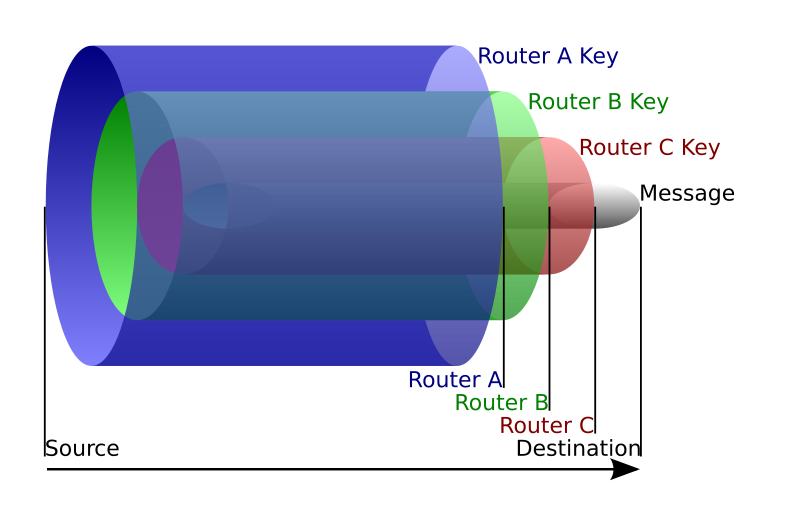
\includegraphics[width=\textwidth]{onion_diagram}
 \caption[Caption for LOF]{Diagram przedstawiający przykładową wiadomość przesyłaną przez obwód\footnotemark.}
 \label{rys:onion_diagram}
\end{figure}
\footnotetext{\url{https://upload.wikimedia.org/wikipedia/commons/e/e1/Onion_diagram.svg}}

\subsection{Komórki}\paragraph{}
Przesyłaną jednostką danych w~Trasowaniu Cebulowym jest tzw. komórka. Ma ona stałą długość 512 bajtów i~składa się z~nagłówka oraz przesyłanej treści. Długość nagłówka jest uzależniona od typu komórki. Może mieć on 3 lub 14 bajtów. Najważniejszymi składowymi nagłówka jest identyfikator obwodu oraz polecenie. Rysunek \ref{rys:cell} przedstawia wygląd komórki.

Pierwsze 2 bajty są zajmowane przez wcześniej wspomniany identyfikator obwodu. Jest on wymagany, gdyż w~pojedyńczym połączeniu pomiędzy poszczególnymi węzłami może zostać ustanowionych wiele obwodów i~każdy węzeł musi wiedzieć do którego z~nich należy komórka.

Kolejny zajmowany bajt przeznaczony jest na polecenie, dzięki któremu węzeł, który otrzyma komórkę, będzie w~stanie zinterpretować ją w~odpowiedni sposób. Wszystkie polecenia można podzielić na dwa typy, kontrolne oraz przekazujące. Do tych pierwszych należą \textit{padding}, \textit{create} oraz \textit{destroy}. Służą one kolejno do utrzymywania połączeń, ustanawiania nowych obwodów oraz niszczenia ich, z~koleji poleceniem mówiącym nam o~tym, że mamy do czynienia z~komórką przekazującą jest \textit{relay}.

Struktura komórki posiadającej polecenie przekazujące różni się od komórek z~poleceniem kontrolnym tym, że pierwsze 11 bajtów treści komórki traktowane jest jako rozszerzenie jej nagłówka. Pierwsze 2 bajty tego rozszerzenia przeznaczone są na identyfikator strumienia, który jest stosowany ze względu na to, że pojedyńczy strumień może zostać zmultipleksowany na wiele obwodów, więc potrzebny jest mechanizm pozwalający odróżnić do jakiego strumienia w~obwodzie należy komórka. Kolejne 6 bajtów zajmuje suma kontrolna, stworzona za pomocą funkcji skrótu SHA-1, pozwalająca na sprawdzenie integralności przesyłanych danych. Kolejne pole nagłówka określa długość przesyłanej treści, a~ostatni bajt definiuje odpowiednie polecenie komórki przekazującej, które może mieć następujące wartości:

\begin{itemize}
\setlength\itemsep{0mm}
 \item \textit{relay data} - przesyłanie danych w~strumieniu
 \item \textit{relay begin} - otwarcie strumienia
 \item \textit{relay end} - bezpieczne zamknięcie strumienia
 \item \textit{relay teardown} - zamknięcie uszkodzonego strumienia
 \item \textit{relay connected} - powiadomienie proxy nadawcy o~rozpoczęciu przekazywania
 \item \textit{relay extend} - rozszerzenie obwodu o~nowy węzeł
 \item \textit{relay extended} - potwierdzenie rozszerzenia obwodu
 \item \textit{relay truncate} - zamknięcie części obwodu
 \item \textit{relay truncated} - potwierdzenie zamknięcia części obwodu
 \item \textit{relay sendme} - kontrola przeciążenia
 \item \textit{relay drop} - implementacja atrap dalekiego zasięgu\footnote{https://svn.torproject.org/svn/projects/design-paper/tor-design.pdf\label{link:tor-design}}
\end{itemize}

\begin{figure}
 \centering
 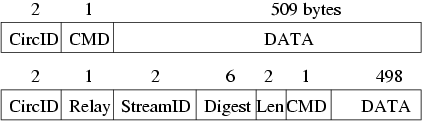
\includegraphics[width=\textwidth]{cell-struct}
 \caption[Caption for LOR]{Struktura komórki Trasowania Cebulowego typu kontrolnego (u góry) oraz przekazującego.\footnotemark}
 \label{rys:cell}
\end{figure}
\footnotetext{https://svn.torproject.org/svn/projects/design-paper/cell-struct.png}

\subsection{Proces tworzenia obwodu}\paragraph{}
Wybrane przez użytkownika serwery pośredniczące, przez które przekierowywana jest wiadomość tworzą tzw. obwód. Proces tworzenia takiego obwodu przebiega w~sposób iteracyjny. Załóżmy, że Alice jest nadawcą, Bob pierwszym, a~Carol drugim i~jednocześnie ostatnim węzłem w~obwodzie:
\begin{enumerate}
 \item Alice w~celu utworzenia połączenia z~Bobem, wysyła do niego wiadomość z~poleceniem \textit{create}. W~nagłówku wiadomości znajduje się również wybrany przez Alice, nieużywany pomiędzy nią, a Bobem identyfikator obwodu. Treścią wiadomości jest pierwsza część procesu  Diffiego-Hellmana, służącego do uzgadniania klucza symetrycznego. Komórka jest zaszyfrowana za pomocą algorytmu RSA, przy użyciu klucza publicznego Boba.
 \item Bob na podstawie otrzymanej od Alice wiadomości oraz własnych danych generuje klucz, a~następnie w~celu finalizacji procesu uzgadniania klucza wysyła do Alice wiadomość z~poleceniem \textit{created}, której treścią jest drugą część procesu, oraz skrót wygenerowanego klucza.
 \item Alice generuje klucz, a~następnie porównuje jego skrót z~tym otrzymanym od Boba. Jeśli oba skróty się zgadzają oznacza to, że Alice i~Bob posiadają ten sam klucz symetryczny, za pomocą którego będą szyfrowane oraz odszyfrowywane przesyłane między nimi wiadomości.
 \item Alice w~celu rozszerzenia obwodu o~kolejny węzeł wysyła do Boba wiadomość z~poleceniem \textit{relay extend}, posiadającą adres Carol oraz połowę procesu uzgadniania klucza symetrycznego.
 \item Bob tworzy nową wiadomość zawierającą polecenie \textit{create} oraz nieużywany między nim a~Carol identyfikator obwodu, a~następnie pakuje do niej treść wiadomości otrzymanej od Alice i~wysyła ją do Carol.
 \item Po otrzymaniu wiadomości Carol wysyła do Boba wiadomość z~poleceniem \textit{created}, której treścią jest drugi etap procesu uzgadniania klucza symetrycznego między nią a~Alice.
 \item Bob oraz Carol mają zapisane w~swoich tablicach informacje o~utworzonych połączeniach. Dodatkowo Bob powiązuje ze sobą identyfikator połączenia Alice z~Carol, dzięki czemu wszystkie wiadomości od Alice będą przekierowywane do Carol i~na odwrót\footnote{https://www.onion-router.net/Publications/IH-1996.pdf\label{link:hiding-information}}. Po tym, w~celu powiadomienia o~pomyślnym rozszerzeniu obwodu oraz finalizacji procesu uzgadniania klucza, do Alice zostaje wysłana wiadomość z~poleceniem \textit{relay extended} z~treścią poprzednio otrzymanej wiadomości od Carol.
 \item Alice generuje klucz symetryczny, identyczny z~tym posiadanym przez Carol. Od tego momentu obwód jest rozszerzony o~nowy węzeł.
 \item W~celu dalszego rozszerzania obwodu powyższy proces może być powtarzany, z~uwzględnieniem zwiększenia długości obwodu o~nowy węzeł w~każdym etapie rozszerzania.
\end{enumerate}

Powyższy proces został zilustrowany na rysunku \ref{rys:circuit}. H(Kx) oznacza skrót SHA-1 klucza symetrycznego współdzielonego z~węzłem x, a $g^{x_z}$ oraz $g^{y_z}$ oznaczają pierwszą oraz drugą część procesu uzgadniania klucza z~węzłem z. Dodatkowo poniżej przerywanej linii widoczny jest proces połączenia ze stroną internetową przy wykorzystaniu Trasowania Cebulowego. 

\begin{figure}
 \centering
 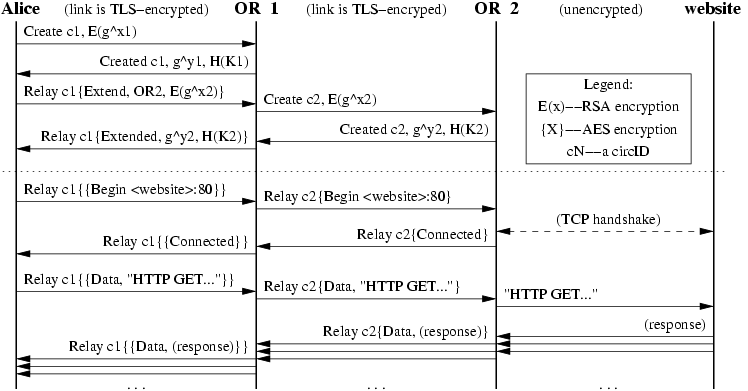
\includegraphics[width=\textwidth]{interaction}
 \caption[Caption for LOR]{Przykładowy przebieg tworzenia obwodu oraz komunikacji ze stroną internetową z~wykorzystaniem Trasowania Cebulowego.\footnotemark}
 \label{rys:circuit}
\end{figure}
\footnotetext{https://svn.torproject.org/svn/projects/design-paper/interaction.png}

W~celu połączenia się z~przykładową witryną internetową nadawca szyfruje zapytanie za pomocą wcześniej uzgodnionych kluczy symetrycznych serwerów pośredniczących, a~następnie przesyła je przez obwód. Do nawiązania połączenia wykorzystywana jest komórka zawierająca polecenie \textit{relay begin} wraz z~nowym nieużywanym identyfikatorem strumienia. Ostatni węzeł, po odebraniu wiadomości, w~imieniu inicjatora nawiązuje połączenie z~witryną, a~następnie odsyła do nadawcy komórkę \textit{relay connected}. Po nawiązaniu połączenia, każde zapytanie pakowane jest w~komórkę zawierającą polecenie \textit{relay data}, która jest szyfrowana i~przesyłana przez obwód. Przy każdym przeskoku każdy kolejny węzeł zdejmuje warstwę przy użyciu współdzielonego między nim oraz nadawcą wiadomości klucza symetrycznego, aż niezaszyfrowana wiadomość trafi do serwera docelowego. Odpowiedź odbiorcy przebiega w~odwrotnej kolejności. Przy każdym przeskoku każdy z~węzłów dodaje jedną warstwę szyfru, co powoduje, że do nadawcy trafia wielokrotnie zaszyfrowana wiadomość. Oprogramowanie inicjatora komunikacji musi zdjąć wszystkie warstwy szyfru, zanim prawidłowa odpowiedź trafi do odpowiedniego programu w~systemie\textsuperscript{\ref{link:tor-design}}.

\subsection{Padding}\paragraph{}
Wraz ze zdjęciem każdej warstwy rozmiar wiadomości ulega zmniejszeniu. Osoba analizująca pakiety w~sieci mogłaby na podstawie długości przesyłanych komórek ustalić położenie danego węzła w~obwodzie. Aby temu zapobiec stosuje się tzw. padding, czyli wypełnienie pozostałego wolnego miejsca w~komórce losowymi danymi. Przy każdym przeskoku w~obwodzie każdy węzeł dodawaje odpowiednią ilość paddingu. Jeżeli komórka jest przesyłana w~stronę inicjatora połączenia, padding musi być usuwany wraz z~każdym przeskokiem komórki w~obwodzie. W~przypadku niektórych komórek np. tych zawierających polecenie \textit{destroy}, padding zajmuje całą treść wiadomości\textsuperscript{\ref{link:hiding-information}}.

\subsection{Niszczenie obwodów}\paragraph{}
Obwód może zostać zniszczony przez każdy z~węzłów, który się w~nim znajduje. W~takiej sytuacji tworzona jest komórka zawierająca polecenie \textit{destroy} oraz identyfikator obwodu, który ma zostać zniszczony. Treść takiej komórki jest pusta. Następnie taka komórka zostaje wysłana do obu sąsiednich węzłów. Każdy z~nich ma obowiązek przekazać taką komórkę w~odpowiednim kierunku obwodu, a~następnie usunąć ze swojej tablicy wpisy dotyczące tego obwodu\textsuperscript{\ref{link:hiding-information}}.

\subsection{Serwery katalogowe}\paragraph{}
Klient sieci Tor musi posiadać aktualną listę serwerów pośredniczących, wraz z~ich kluczami publicznymi, oraz aktualnym stanem. Pierwotnie te informacje miały być udostępniane na zasadzie peer-to-peer. Oznacza to, że węzły miały wymieniać się posiadanym o~sobie danymi. Ten sposób okazał się jednak nieodpowiedni ze względów bezpieczeństwa. Niektóre węzły w~sieci mogły posiadać różne informacje o~tych samych serwerach pośredniczących, co mogło umożliwić potencjalnemu napastnikowi określenie położenia węzła w~sieci. Poza tym wymiana tych danych między węzłami spowodowałaby niepotrzebne obciążenie sieci. Zdecydowano więc, że informacje te będą przechowywane w~centralnych serwerach zwanych serwerami katalogowymi. Domyślnie oprogramowanie klienckie posiada listę wszystkich tych serwerów, od których raz na jakiś czas pobierane są informacje o~wszystkich węzłach pośredniczących występujących w~sieci Tor. Każdy taki serwer katalogowy jest serwerem HTTP. Pozwala to na proste udostępnianie oraz pobieranie informacji. Każdy serwer, który udostępnia swoje dane serwerowi katalogowemu musi wcześniej je podpisać za pomocą swojego klucza. Ta sama sytuacja dotyczy serwera katalogowego. Zanim zebrane przez serwer katalogowy infromacje zostaną udostępnione klientom, muszą zostać podpisane przez serwer katalogowy przy użyciu swojego klucza prywatnego. Ma to uniemożliwić potencjalnemu napastnikowi na podstawienie własnego serwera pośredniczącego lub katalogowego\textsuperscript{\ref{link:tor-design}}.